\documentclass[12pt]{article}

\usepackage{sbc-template}
\usepackage{graphicx,url,setspace,subfig, float}
\usepackage[utf8]{inputenc}
\usepackage[brazil]{babel}

\sloppy

\title{MAC5753 -- Sistemas Operacionais -- 2s2020\\ EP2}

\author{Guilherme Werneck de Oliveira\inst{1}}

\address{Departamento de Ciência da Computação -- Universidade de São Paulo (USP)\\
  Rua do Matão, 1010 - CEP 05508-090 - São Paulo - SP}

\begin{document}

\maketitle

\begin{abstract}
  This report describes the development and the results obtained from experiments performed with shared memory. An elimination run simulator with a multithreading approach was developed. The experiments carried out considered two main contexts, the main memory consumption and the program execution time considering different track configurations and different amounts of cyclists. The results presented showed a proportional increase in the execution time according to the increase in the number of cyclists, as well as the increase in the track. Also, they showed that the main memory consumption was constant according to the different track configurations.
\end{abstract}

\begin{resumo}
  Este relatório descreve o desenvolvimento e os resultados aferidos de experimentos realizados com memória compartilhada. Foi desenvolvido um simulador de corrida por eliminação com uma abordagem multithreading. Os experimentos realizados consideraram dois principais contextos, o consumo de memória principal e o tempo de execução do programa considerando diferentes configurações de pista e diferentes quantidades de ciclistas. Os resultados apresentados mostraram um aumento proporcional do tempo de execução de acordo com o aumento da quantidade de ciclistas, assim como o aumento da pista. Também, mostraram que o consumo de memória principal foi constante de acordo com as diferentes configurações de pista.
\end{resumo}


\section{Introdução}

O gerenciamento de memória é um dos mecanismos necessários para todo e qualquer sistema operacional. Ele permite que a memória principal (RAM) seja alocada e desalocada de forma eficiente durante o inicio, a execução e o termino de programas.

Em sistemas operacionais multiprogramados, onde vários programas concorrem simultaneamente pelo mesmo \textit{hardware}, é possível encontrar um recurso chamado de \textbf{memória virtual}. Esse recurso permite que cada programa tenha seu próprio espaço de endereçamento dividido em blocos, conhecidos como \textbf{páginas}. \cite{tanenbaum:16}.

Na criação de um novo processo, um determinado espaço de endereçamento é reservado para ele. Quando esse processo utiliza algum mecanismo de processamento paralelo de tarefas, por exemplo \textit{threading}, esse espaço de endereçamento é compartilhado entre todos os recursos do mesmo processo. Uma das vantagens dessa estratégia é a redução da complexidade na implementação e na manipulação de acessos a recursos compartilhados, não necessitando realizar comunicações entre processos diferentes. No entanto, é necessária a criação e a utilização de abordagens de acesso exclusivo a um recurso compartilhado como, por exemplo, uma estrutura alocada na memória principal.

Este trabalho mostra o desenvolvimento de um simulador de corrida e os resultados de testes aplicados, com o principal objetivo de utilizar o compartilhamento de memória principal (a pista) por meio de \textit{mutithreads} (os ciclistas).

\section{Descrição do Problema} \label{sec:firstpage}

A tarefa solicitada neste segundo exercício prático (EP2) da disciplina de Sistemas Operacionais do 2º semestre de 2020 solicita a implementação de um simulador de corrida de ciclismo na modalidade por eliminação.

A corrida por eliminação se inicia com os ciclistas lado a lado em um velódromo. A cada duas voltas, o ciclista que completar a última volta na última posição é eliminado. Assim, a prova é finalizada quando sobrar apenas um ciclista.

O simulador deve considerar um velódromo com $d$ metros e $n$ ciclistas no início da prova, onde $(d>249, 5<n\leq 5\cdot d)$, no máximo dez ciclistas podem estar lado a lado e que cada ciclista ocupa um metro de comprimento da pista.

Como entrada, o simulador deve receber, via linha de comando, os dois números inteiros: $d$ $n$.

\section{Descrição da Solução}

O código-fonte e os resultados aferidos estão disponíveis em \url{github.com/werneckg/mestrado/tree/master/SO/EP2}. A implementação do código-fonte foi estruturada da seguinte forma:
\begin{itemize}
	\item ep2.h, arquivo contendo o cabeçalho das funções utilizadas pelo ep2;
	\item ep2.c, implementação das funções utilizadas pelo ep2;
	\item main-ep2.c, arquivo contendo a implementação da função principal do ep2.
\end{itemize}

\subsection{A Pista}

O simulador considera, para o desenvolvimento da pista, um vetor global com acesso simultâneo realizado pelos ciclistas, representados por \textit{threads}. Para maiores detalhes sobre a implementação dos ciclistas, veja a seção \ref{subsec:os-ciclistas}.

A pista é implementada por meio de um vetor onde cada metro, representado pela posição do vetor, é uma estrutura chamada \textit{tTrack} como ilustra a Figura~\ref{fig:track}. Essa estrutura contém um vetor circular com dez posições que representa a quantidade de linhas da pista, juntamente com um atributo que controla a próxima posição do vetor em que um ciclista pode colocar sua identificação. Como o vetor pista é uma estrutura de dados compartilhada entre todos os ciclistas, o controle do acesso posição a posição, representada pelos metros da pista, é realizado através de exclusão mútua, \textit{mutex} \cite{robbins:00}.

Quando um ciclista acessa um determinado metro da pista, primeiramente ele remove sua identificação da linha da pista do metro anterior que esteve. Após isso, ele acessa a linha que está livre, vetor circular de linhas, no metro seguinte. Por fim, o ciclista incrementa a posição do vetor circular de linhas para que o próximo ciclista possa acessar uma linha livre naquele metro.

\begin{figure}[H]
	\centering
	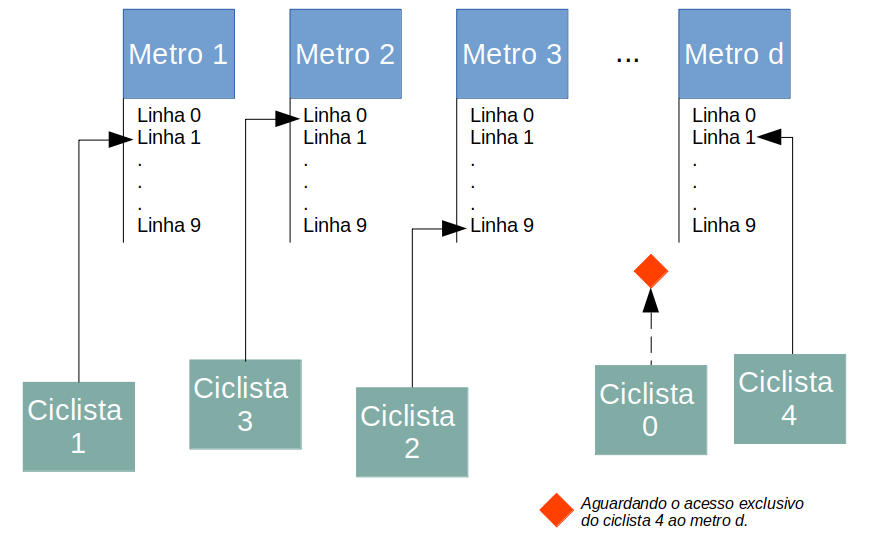
\includegraphics[width=.9\textwidth]{track.png}
	\caption{Representação da estrutura da pista.}
	\label{fig:track}
\end{figure}

\subsection{Os Ciclistas}
\label{subsec:os-ciclistas}

Cada ciclista possui uma identificação e é representado por uma \textit{thread} de mesma identificação. Dessa forma, o simulador cria e executa a mesma quantidade de \textit{threads} informada como a quantidade de ciclistas na linha de comando para a execução da corrida.

O simulador cria um vetor de ciclistas onde cada um é representado por uma estrutura chamada \textit{tCyclist} como ilustrado na Figura~\ref{fig:cyclist}. Essa estrutura contém o número do ciclista, seu estado em determinada volta, sua velocidade para cada volta, o metro e a linha atuais da pista, sua posição final na corrida, a volta em que quebrou quando aplicável, seu tempo na volta e seu tempo final na corrida.

\begin{figure}[H]
	\centering
	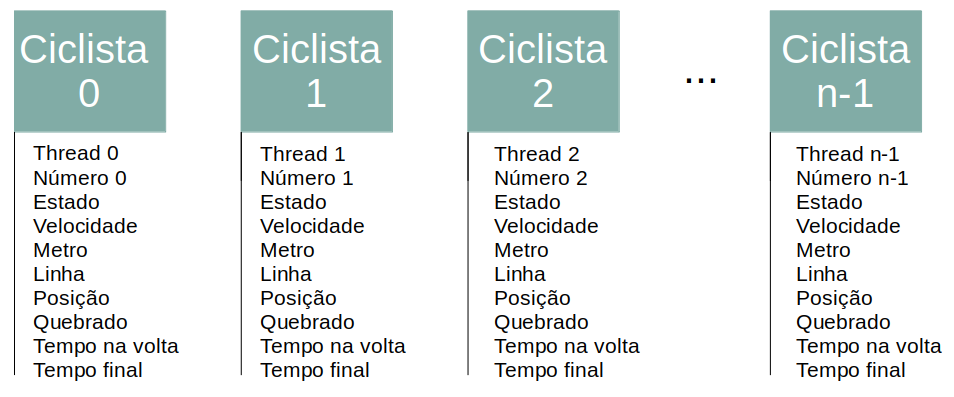
\includegraphics[width=.9\textwidth]{cyclist.png}
	\caption{Representação da estrutura do ciclista.}
	\label{fig:cyclist}
\end{figure}


\subsection{A Corrida}

Como a corrida por eliminação considera a eliminação do último ciclista ao cruzar a linha de chegada a cada duas voltas, o simulador implementa uma barreira \cite{ibm:20}, Figura~\ref{fig:barrier}, com o intuito de sincronizar todas as \textit{threads}, ou ciclistas, ao final de duas voltas. Após a sincronização dos ciclistas, o processo de eliminação é executado.

Todo ciclista, quando é criado, tem sua variável local de tempo iniciada pela função \textit{clock()}. Quando corre uma determinada volta, seu estado é alterado para ``correndo" e sua velocidade é determinada de acordo com os requisitos solicitados na descrição do EP. Após  a definição da velocidade do ciclista, a função \textit{usleep()} é executada, considerando sua velocidade, antes do incremento da variável que controla os metros andados pelo ciclista. No final da volta, sua variável de tempo em determinada volta é computada para ser utilizada no processo de eliminação.

\begin{figure}[H]
	\centering
	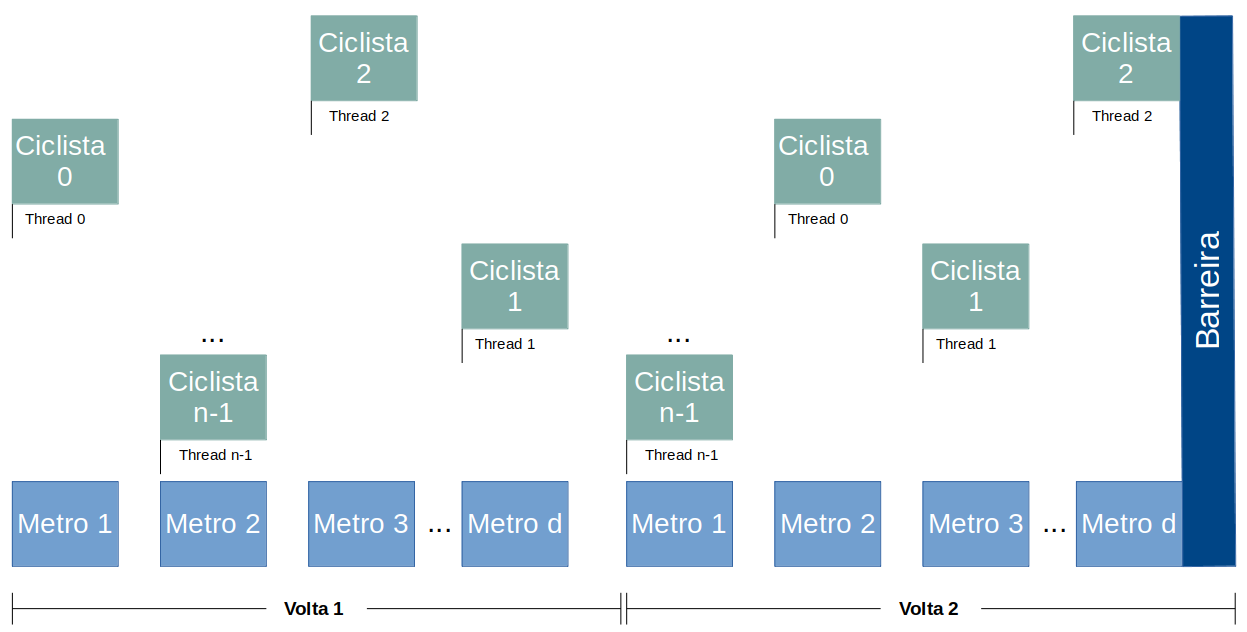
\includegraphics[width=1\textwidth]{barrier.png}
	\caption{Representação da estrutura de barreira.}
	\label{fig:barrier}
\end{figure}

O processo de eliminação realiza uma eleição de qual ciclista alcançou o maior tempo no final de duas voltas. Após essa eleição, o ciclista selecionado atualiza seu estado para ``eliminado", decrementa o contador da barreira, atualiza sua posição final, destrói a barreira e cria uma nova com o novo número de cilistas para as voltas seguintes e finaliza sua \textit{thread}. Essa abordagem de implementação garante que todas as \textit{threads} sejam finalizadas no mesmo momento em que o ciclista foi eliminado ou quebrado, fazendo com que o recurso computacional de processamento alocado para o processo seja liberado.

Assim como a eliminação do ciclista, o simulador considera que o ciclista pode ter quebrado na última volta em que correu. Nesse caso, a \textit{thread} do ciclista é finalizada e barreira é atualizada.

A cada volta da corrida, as posições de cada ciclista são apresentadas juntamente com seus respectivos tempos contabilizados. Por fim, ao termino da corrida, o ranqueamento final é apresentado contendo também as posições de cada ciclista, seus tempos e, quando quebrado, a volta em que quebrou.


\section{Resultados Obtidos}

Os resultados apresentados foram obtidos a partir da execução do simulador de corrida em uma máquina física com processador Intel® Core i5 com 4 CPUs, 6 GB de memória RAM e sistema operacional Ubuntu 20.04.1 LTS.

Os valores apresentados nos gráficos a seguir foram obtidos a partir de 30 execuções do simulador de corrida para cada uma das instâncias e foram aferidos com um intervalo de 95\% de confiança. A quantidade de ciclistas e o tamanho da pista foram definidos com base em parâmetros próximos ao de uma corrida real. As instâncias utilizadas foram:

\begin{itemize}
	\item Poucos ciclistas (13): pista com 250, 700 e 1200 metros;
	\item Médios ciclistas (21): pista com 250, 700 e 1200 metros;
	\item Muitos ciclistas (55): pista com 250, 700 e 1200 metros.
\end{itemize}

\subsection{Tempo de Execução}

A aferição do tempo de execução do simulador foi realizada a partir da execução da função \textit{time} juntamente com o binário do programa, por exemplo, \textit{time ./ep2 1200 55}.

O gráfico ilustrado na Figura~\ref{fig:time} apresenta o tempo de execução do simulador para as instâncias com poucos, médios e muitos ciclistas em diferentes tamanhos de pista. O primeiro fato observado foi o aumento do tempo de execução de forma proporcional ao aumento do número de ciclistas para todas as configurações de pista. Esse aumento representou cerca de 87\% para poucos, 90\% para médios e 87\% para muitos ciclistas nas pistas de 250, 700 e 1200 metros respectivamente. Isso se deve ao fato da criação e execução de um número maior de \textit{threads} e, consequentemente, o aumento do número de voltas necessárias para a definição de um vencedor.

\begin{figure}[H]
	\centering
	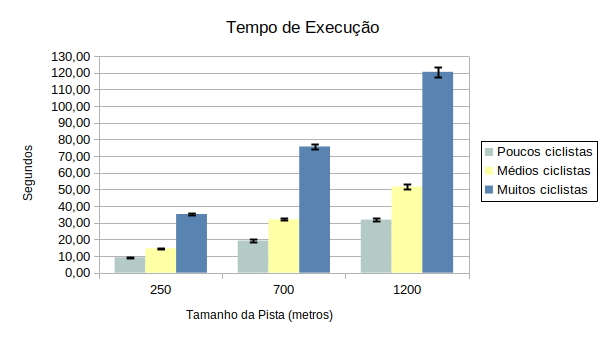
\includegraphics[width=1\textwidth]{time.png}
	\caption{Tempo de execução do simulador de corrida.}
	\label{fig:time}
\end{figure}

Outro fato importante observado em todas as instâncias, foi a redução significativa do tempo de execução do simulador, em média 17\%, nos casos em que houveram de 4 a 18 ciclistas quebrados na corrida.

\subsection{Consumo de Memória}

A aferição do consumo de memória principal foi realizada a partir da observação do processo gerado para o simulador por meio do comando \textit{top}. Contabilizado em KB, foram observados os valores dos atributos RES, que representa o consumo de memória física real pelo processo e SHR, que representa a quantidade de memória compartilhada pelo processo.

Foi observado um aumento no consumo de memória RES de cerca de 18,5\% e SHR de 10\% entre poucos e médios ciclistas para todos os tamanhos de pista, como mostra a Figura~\ref{fig:cm_pc} e a Figura~\ref{fig:cm_mc}. Já entre médios e muitos ciclistas, Figura~\ref{fig:cm_mc} e Figura~\ref{fig:cm_mmc}, o aumento representou cerca de 56\% de memória RES e 0,2\% SHR. Esse crescimento era esperado uma vez que aumentado o número de ciclistas, \textit{threads}, há maior alocação de variáveis utilizadas pelo processo.

Por fim, foi observado uma estabilidade no consumo de memória de acordo com o aumento do tamanho da pista para todas as quantidades de ciclistas. Esse fato pode estar relacionado a escolha do tamanho das pistas para o teste, que nesse caso, foram poucos distantes entre si.

\begin{figure}[H]
	\centering
	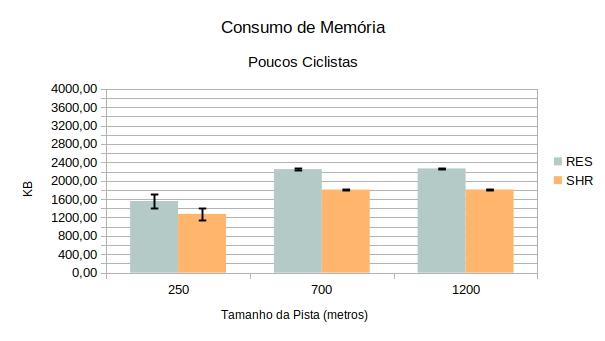
\includegraphics[width=1\textwidth]{cm_pc.png}
	\caption{Consumo de memória do simulador de corrida para poucos ciclistas.}
	\label{fig:cm_pc}
\end{figure}

\begin{figure}
	\centering
	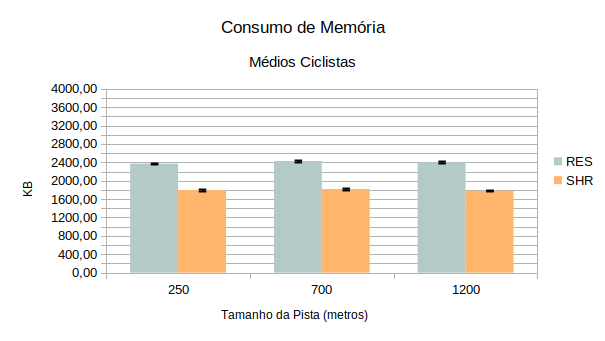
\includegraphics[width=1\textwidth]{cm_mc.png}
	\caption{Consumo de memória do simulador de corrida para médios ciclistas.}
	\label{fig:cm_mc}
\end{figure}

\begin{figure}
	\centering
	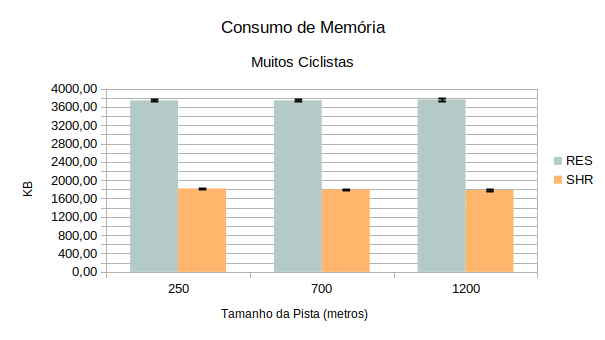
\includegraphics[width=1\textwidth]{cm_mmc.png}
	\caption{Consumo de memória do simulador de corrida para muitos ciclistas.}
	\label{fig:cm_mmc}
\end{figure}


\clearpage

\bibliographystyle{sbc}
\bibliography{sbc-template}

\end{document}
